\documentclass[11pt]{article}

\usepackage{a4wide}
\usepackage[utf8]{inputenc}
\usepackage[russian]{babel}
\usepackage{graphicx}
\usepackage{amsmath}
\usepackage{float}
\usepackage{hyperref}

\DeclareMathOperator{\sinc}{sinc}
\DeclareMathOperator{\arctg}{arctg}

\begin{document}

\thispagestyle{empty}

\begin{center}
\ \vspace{-3cm}

\includegraphics[width=0.5\textwidth]{msu.eps}\\
{\scshape Московский государственный университет имени М.~В.~Ломоносова}\\
Факультет вычислительной математики и кибернетики\\
Кафедра системного анализа

\vfill

{\LARGE Отчет по практикуму}

\vspace{1cm}

{\Huge\bfseries <<Численное решение краевой задачи при помощи БПФ>>}
\end{center}

\vspace{1cm}

\begin{flushright}
  \large
  \textit{Студент 315 группы}\\
  М.\,В.~Миловидов

  \vspace{5mm}

  \textit{Руководитель практикума}\\
  к.ф.-м.н., доцент П.\,А.~Точилин
\end{flushright}

\vfill

\begin{center}
Москва, 2024
\end{center}

\newpage
\section{Постановка задачи}

Рассмотрим краевую задачу:
\begin{equation}
\begin{cases}
    u_{xx}(x, y) + u_{yy}(x, y) - \mu \cdot u(x, y) = f(x, y), & (x, y) \in [0, 1] \times [0, 1], \\
    u(x, 0) \equiv u(x, 1) \equiv \xi(x), \\
    u(0, y) \equiv u(1, y) \equiv \eta(y).
\end{cases}
\end{equation}
$\mu > 0$, $f \in C^1([0, 1] \times [0, 1]), \xi, \eta \in C^1([0, 1]), \xi(0) = \xi(1) = \eta(0) = \eta(1)$.
Для этой краевой задачи рассматривается разностная схема:
\begin{equation}
\begin{cases}
    \frac{y_{k+1, \ell} - 2y_{k, \ell} + y_{k-1, \ell}}{h_x^2}+ \frac{y_{k, \ell+1} - 2y_{k, \ell} + y_{k, \ell-1}}{h_y^2}-\mu y_{k, \ell} = \varphi_{k,\ell} \\
     y_{k, 0} = y_{k, N} = \xi_k, y_{0, \ell}=y_{M, \ell}=\eta_\ell, k = \overline{1, M-1}, \ell = \overline{1, N-1}.
\end{cases}
\end{equation}
Здесь $h_x=1/M, h_y = 1/N$ - значения $y_{k,\ell}$ аппроксимирующие функцию $u(x, y)$ в узлах сетки для $\ x_k=k/M, \ y_\ell=\ell / N, \ \varphi_{k, \ell}=f(x_k, y_\ell), \ \xi_k=\xi(x_k),\ \eta_\ell=\eta(y_\ell)$

\vspace{0.5cm} 

Для функции
\[
f(x, y) = xe^{-2x}\cos(x) + (2+y)\cos(2y).
\]
реализовать в Matlab функцию fGiven, так чтобы можно было взять fHandle=@fGiven, и решить задачу (1) аналитически. Для этого, учитывая что $f(x, y) = f_1(x) + f_2(y)$, взять $u(x, y) = u_1(x) + u_2(y)$ и решить аналитически соответствующие дифференциальные уравнения для $u_1$ и
$u_2$ с краевыми условиями $u_1(0) = u_1(1) = u_1^0$ и $u_2(0) = u_2(1) = u_2^0$.
Аналитическое решение задачи (1) поместить в
тело функции uAnalytical(xMat,yMat,u1Zero,u2Zero,mu), где xMat и yMat соответствуют матрицам одного размера со
значениями переменных x и y, а u1Zero, u2Zero и mu дают значения скалярных параметров $u_1^0, u_2^0$ и $\mu$, соответственно.
Написать функцию uNumerical(u1Zero,u2Zero,mu,M,N), которая передает на вход функции solveDirichlet параметры
\begin{itemize}
    \item fHandle=@fGiven,
    \item xiHandle=@(x)uAnalytical(x,zeros(size(x)),u1Zero,u2Zero,mu),
    \item etaHandle=@(y)uAnalytical(zeros(size(y)),y,u1Zero,u2Zero,mu)
\end{itemize}
и возвращает результат работы solveDirichlet (то есть краевые условия в (1) берутся прямо из полученного аналити-
ческого решения). График аналитического решения сравнить с графиком приближенного решения, полученного из (2)
при различных M и N , нарисовать график разности между численным и аналитическим решением.

\newpage
\section{Решение задачи}

Рассмотрим двумерное дискретное преобразование Фурье для $y_{k, \ell}$ и $\varphi_{k, \ell}$ по данной сетке:
\[
y_{k,\ell} = \sum_{p=0}^{M-1} \sum_{q=0}^{N-1} a_{p,q} e^{-2\pi i \left( \frac{kp}{M} + \frac{lq}{N} \right)}
\]
\[
\varphi_{k,\ell} =  \sum_{p=0}^{M-1} \sum_{q=0}^{N-1} b_{p,q} e^{-2\pi i \left( \frac{kp}{M} + \frac{lq}{N} \right)}
\]
\[p = \overline{1, M-1},\ q = \overline{1, N-1}.\]
Применим его к разностной схеме (2):
\[
M^2\left(\sum_{p=0}^{M-1} \sum_{q=0}^{N-1} a_{p,q} e^{-2\pi i \left( \frac{(k+1)p}{M} + \frac{lq}{N} \right) } -2 \sum_{p=0}^{M-1} \sum_{q=0}^{N-1} a_{p,q} e^{-2\pi i \left( \frac{kp}{M} + \frac{lq}{N} \right)} + \sum_{p=0}^{M-1} \sum_{q=0}^{N-1} a_{p,q} e^{-2\pi i \left( \frac{(k-1)p}{M} + \frac{lq}{N} \right)}\right) +\
\]
\[
+\ N^2\left( \sum_{p=0}^{M-1} \sum_{q=0}^{N-1} a_{p,q} e^{-2\pi i \left( \frac{kp}{M} + \frac{(l+1)q}{N} \right)} -2\sum_{p=0}^{M-1} \sum_{q=0}^{N-1} a_{p,q} e^{-2\pi i \left( \frac{kp}{M} + \frac{lq}{N} \right)} + \sum_{p=0}^{M-1} \sum_{q=0}^{N-1} a_{p,q} e^{-2\pi i \left( \frac{kp}{M} + \frac{(l-1)q}{N} \right)} \right) -\
\]
\[
- \ \mu \sum_{p=0}^{M-1} \sum_{q=0}^{N-1} a_{p,q} e^{-2\pi i \left( \frac{kp}{M} + \frac{lq}{N} \right)} = \sum_{p=0}^{M-1} \sum_{q=0}^{N-1} b_{p,q} e^{-2\pi i \left( \frac{kp}{M} + \frac{lq}{N} \right)}.
\]
\[
\sum_{p=0}^{M-1} \sum_{q=0}^{N-1} a_{p,q} e^{-2\pi i \left( \frac{kp}{M} + \frac{lq}{N} \right)} \left( M^2 \left( e^{\frac{-2 \pi i p}{M}} - 2 + e^{\frac{2 \pi i p}{M}} \right) + N^2 \left( e^{\frac{-2 \pi i q}{N}} - 2 + e^{\frac{2 \pi i q}{N}} \right) - \mu \right) =\
\]
\[
= \sum_{p=0}^{M-1} \sum_{q=0}^{N-1} b_{p,q} e^{-2\pi i \left( \frac{kp}{M} + \frac{lq}{N} \right)}.
\]
Обозначим выражение в скобках за $c_{p, q}$:
\[
c_{p, q} = M^2 \left( e^{\frac{-2 \pi i p}{M}} - 2 + e^{\frac{2 \pi i p}{M}} \right) + N^2 \left( e^{\frac{-2 \pi i q}{N}} - 2 + e^{\frac{2 \pi i q}{N}} \right) - \mu.
\]
Таким образом $\forall \ p = \overline{1, M-1},\ q = \overline{1, N-1}$ имеем $a_{p, q} = \frac{b_{p, q}}{c_{p, q}}$.
\\
ОДПФ для $b_{p, q}$:
\[
b_{p, q} = \frac{1}{MN} \sum_{p=0}^{M-1} \sum_{q=0}^{N-1} \varphi_{k, \ell} e^{2\pi i \left( \frac{kp}{M} + \frac{lq}{N} \right)} = 
\]
\[
= \frac{1}{MN} \left( \varphi_{0,0} + \sum_{k=1}^{M-1} \varphi_{k,0} e^{2\pi i \frac{kp}{M}} + \sum_{\ell=1}^{N-1} \varphi_{0,\ell} e^{2\pi i \frac{\ell q}{N}} + \sum_{k=1}^{M-1} \sum_{\ell=1}^{N-1} \varphi_{k,\ell} e^{2\pi i \left( \frac{kp}{M} + \frac{\ell q}{N} \right)} \right) = b_{p,q} = \varphi_0 + \tilde{b_{p,q}},
\]
где
\[
\varphi_{0} = \frac{1}{MN} \left( \varphi_{0,0} + \sum_{k=1}^{M-1} \varphi_{k,0} e^{2\pi i \frac{kp}{M}} + \sum_{\ell=1}^{N-1} \varphi_{0,\ell} e^{2\pi i \frac{\ell q}{N}} \right),
\]
\[
\tilde{b_{p,q}} = \frac{1}{MN} \sum_{k=1}^{M-1} \sum_{\ell=1}^{N-1} \varphi_{k,\ell} e^{2\pi i \left( \frac{kp}{M} + \frac{\ell q}{N} \right)}.
\]
Тогда
\[
a_{p, q} = \frac{\varphi_0}{c_{p, q}} + \frac{\tilde{b_{p,q}}}{c_{p, q}}.
\]
Напишем одномерное ДПФ для функций $\xi, \eta$:
\[
\xi_k = \sum_{p=0}^{M-1} \gamma_p e^{-2\pi i \frac{kp}{M}}, \ k = \overline{1, M-1},
\]
\[
\eta_\ell = \sum_{q=0}^{N-1} \delta_q e^{-2\pi i \frac{\ell q}{N}}, \ \ell = \overline{1, N-1}.
\]
Учтем краевые условия и получим:
\[
y_{k,0} =\xi_k \Rightarrow \sum_{p=0}^{M-1} \sum_{q=0}^{N-1} a_{p,q} e^{-2\pi i \frac{kp}{M}} = \sum_{p=0}^{M-1} \gamma_p e^{-2\pi i \frac{kp}{M}} \Rightarrow \gamma_p = \sum_{q=0}^{N-1} a_{p,q} \ \forall k = \overline{1, M-1}, 
\]
\[
y_{0,\ell} = \eta_\ell \Rightarrow \sum_{p=0}^{M-1} \sum_{q=0}^{N-1} a_{p,q} e^{-2\pi i \frac{\ell q}{N}} =  \sum_{q=0}^{N-1} \delta_q e^{-2\pi i \frac{\ell q}{N}} \Rightarrow \delta_q = \sum_{p=0}^{M-1} a_{p,q} \ \forall \ell = \overline{1, N-1}.
\]
Используя выражение $a_{p, q} = \frac{\varphi_0}{c_{p, q}} + \frac{\tilde{b_{p,q}}}{c_{p, q}}$, получим систему уравнений:
\begin{equation*}
\begin{cases}
\begin{aligned}
&\sum_{q=0}^{N-1}\left(\frac{1}{MNc_{p,q}}\sum_{k=0}^{M-1}\varphi_{k, 0}e^{2\pi i \frac{kp}{M}} + \frac{1}{MNc_{p,q}}\sum_{\ell=1}^{N-1}\varphi_{0, \ell}e^{2\pi i \frac{\ell q}{N}} + \frac{\tilde{b}_{p,q}}{c_{p, q}}\right) = \gamma_p, \ p = \overline{0, M-1},\\
&\sum_{p=0}^{M-1}\left(\frac{1}{MNc_{p,q}}\sum_{k=0}^{M-1}\varphi_{k, 0}e^{2\pi i \frac{kp}{M}} + \frac{1}{MNc_{p,q}}\sum_{\ell=1}^{N-1}\varphi_{0, \ell}e^{2\pi i \frac{\ell q}{N}} + \frac{\tilde{b}_{p,q}}{c_{p, q}}\right) = \delta_q, \ q = \overline{0, N-1}.
\end{aligned}
\end{cases}
\end{equation*}

Преобразуем систему:
\begin{equation*}
\begin{cases}
\begin{aligned}
 &\sum_{k=0}^{M-1}\varphi_{k, 0}\left(\frac{1}{MN}\sum_{q=0}^{N-1}\frac{1}{c_{p,q}}e^{2\pi i \frac{kp}{M}}\right) + \sum_{\ell=1}^{N-1}\varphi_{0, \ell}\left(
\frac{1}{MN}\sum_{q=0}^{N-1}\frac{1}{c_{p,q}}e^{2\pi i \frac{\ell q}{N}}\right) + \sum_{q=0}^{N-1}\frac{\tilde{b}_{p,q}}{c_{p,q}} = \gamma_p, \ p = \overline{0, M-1}\\

&\sum_{k=0}^{M-1}\varphi_{k, 0}\left(\frac{1}{MN}\sum_{p=0}^{M-1}\frac{1}{c_{p,q}}e^{2\pi i \frac{kp}{M}}\right) + \sum_{\ell=1}^{N-1}\varphi_{0, \ell}\left(
\frac{1}{MN}\sum_{p=0}^{M-1}\frac{1}{c_{p,q}}e^{2\pi i \frac{\ell q}{N}}\right) + \sum_{p=0}^{M-1}\frac{\tilde{b}_{p,q}}{c_{p,q}} = \delta_q, \ q = \overline{0, N-1}.
\end{aligned}
\end{cases}
\end{equation*}

Введем обозначения:
$$\theta_{k, p} = \frac{1}{MN}\sum_{q=0}^{N-1}\frac{1}{c_{p,q}}e^{2\pi i \frac{kp}{M}},\ \ \ \tau_{\ell, p} = \frac{1}{MN}\sum_{q=0}^{N-1}\frac{1}{c_{p,q}}e^{2\pi i \frac{\ell q}{N}}.$$

$$\alpha_{k, q} = \frac{1}{MN}\sum_{p=0}^{M-1}\frac{1}{c_{p,q}}e^{2\pi i \frac{kp}{M}},\ \ \ \beta_{\ell, q} = \frac{1}{MN}\sum_{p=0}^{M-1}\frac{1}{c_{p,q}}e^{2\pi i \frac{\ell q}{N}}.$$

Система преобразуется в:
\begin{equation*}
\begin{cases}
\begin{aligned}
&\sum_{k=0}^{M-1}\varphi_{k, 0}\theta_{k, p} + \sum_{\ell=1}^{N-1}\varphi_{0, \ell}\tau_{\ell, p} + \sum_{q=0}^{N-1}\frac{\tilde{b}_{p,q}}{c_{p,q}} = \gamma_p, \ p = \overline{0, M-1}\\

&\sum_{k=0}^{M-1}\varphi_{k, 0}\alpha_{k, q} + \sum_{\ell=1}^{N-1}\varphi_{0, \ell}\beta_{\ell, q} + \sum_{p=0}^{M-1}\frac{\tilde{b}_{p,q}}{c_{p,q}} = \delta_q, \ q = \overline{0, N-1}.
\end{aligned}
\end{cases}
\end{equation*}
Учитывая последнее краевое условие
\[
y_{00} = \xi_0 = \eta_0,
\]
имеем
\[
\sum_{p=0}^{M-1}\gamma_p = \sum_{q=0}^{N-1}\delta_q,
\]
и при добавлении в систему можем исключить одно из уравнений (например при p = 0). В итоге получаем
\begin{equation*}
\begin{cases}
\begin{aligned}
&\sum_{k=0}^{M-1}\varphi_{k, 0}\theta_{k, p} + \sum_{\ell=1}^{N-1}\varphi_{0, \ell}\tau_{\ell, p} + \sum_{q=0}^{N-1}\frac{\tilde{b}_{p,q}}{c_{p,q}} = \gamma_p, \ p = \overline{0, M-1}\\

&\sum_{k=0}^{M-1}\varphi_{k, 0}\alpha_{k, q} + \sum_{\ell=1}^{N-1}\varphi_{0, \ell}\beta_{\ell, q} + \sum_{p=0}^{M-1}\frac{\tilde{b}_{p,q}}{c_{p,q}} = \delta_q, \ q = \overline{0, N-1}.
\end{aligned}
\end{cases}
\end{equation*}
- систему с M + N - 1 уравнениями и M + N - 1 неизвестными $\Rightarrow$ имеющую единственное решение.

Для решения системы

\begin{enumerate}
    \item Вычисляем сетки для известных функций
    \item Находим $c_{p, q}$
    \item При помощи ifft2 от f находим \tilde{b_{p, q}}
    \item Находим $\varphi_0$ через систему
    \item Находим $b_{k, \ell}$ через ifft2
    \item Из получишвегося выражаем $a_{p, q}$ и при помощи fft2 получаем значения функции $\varphi_{k,\ell }$
\end{enumerate}

\newpage
\section{Аналитическое решение}

Для проверки работы алгоритма решим задачу для функции из примера аналитически:

Учитывая, что $f(x, y) = f_1(x) + f_2(y)$, положим $u(x, y) = u_1(x) + u_2(y)$ и решим следующие задачи:

\begin{equation}
\begin{cases}
    u_1''(x) - \mu \cdot u_1(x) = xe^{-2x}\cos(x), x \in [0, 1], \\
    u_1(0) \equiv u_1(1) \equiv u_1^0
\end{cases}
\end{equation}

\begin{equation}
\begin{cases}
    u_2''(y) - \mu \cdot u_2(y) = (2+y)\cos(2y), y \in [0, 1], \\
    u_2(0) \equiv u_2(1) \equiv u_2^0
\end{cases}
\end{equation}

\subsection{Решение для $u_1$}
Запишем решение в виде суммы решения однородной задачи и частного решения неоднородной:
\[
    u_1(x) = u_1^{oo}(x) + u_1^{ch}(x).
\]
Решение однородной задачи, очевидно, имеет вид
\[
    u_1^{oo}(x) = K_1 e^{-\sqrt{\mu}x} + K_2 e^{\sqrt{\mu}x}
\]

Найдем частное решение неоднородной задачи. Будем искать в виде 
\[
    u_1^{ch}(x) = (Ax+B) e^{-2x} \cos(x) + (Cx+D) e^{-2x} \sin(x) = e^{-2x}\left((Ax+B) \cos(x) + (Cx+D) \sin(x)\right).
\]
Тогда
\[
    (u_1^{ch}(x))'' = 4e^{-2x}\left((Ax+B) \cos(x) + (Cx+D) \sin(x)\right) - 
\]
\[
    - 4e^{-2x}\left(A\cos(x) -(Ax+B) \sin(x) + C\sin(x) + (Cx+D) \cos(x)\right) + 
\]
\[
    + e^{-2x}\left(-2A \sin(x) - (Ax+B) \cos(x) + 2C \cos(x) - (Cx+D) \sin(x)\right) = 
\]
\[
    = (3A - 4C)e^{-2x}x\cos(x) + (3C-4A)e^{-2x}x\sin(x) + 
\]
\[
    + (3B - 4A - 4D + 2C)e^{-2x}\cos(x) + (3D + 4B - 4C - 2A)e^{-2x}\sin(x).
\]
\[
    3A - 4C - \mu A - 1 = 0 \Rightarrow\ A = \frac{1 + 4C}{3 - \mu}
\]
\[
    3C-4A-\mu C = 0.\ (3 - \mu)C - 4\frac{1 +4C}{3 - \mu} = 0.\ ((3-\mu)^2 - 16)C = 4 
\]
\[
\Rightarrow C = \frac{4}{(3-\mu)^2 - 16} \Rightarrow A = \frac{1}{3 - \mu}\frac{(3 - \mu)^2 - 16 + 16}{(3-\mu)^2 - 16} = \frac{3 - \mu}{(3-\mu)^2 - 16}
\]
\[
3B - 4A - 4D + 2C - \mu B = 0 \Rightarrow B = \frac{4A -2C + 4D}{3 - \mu}
\]
\[
3D + 4B - 4C - 2A -\mu D = 0.\ (3 - \mu)D + 4 \frac{4A -2C + 4D}{3 - \mu} = 4C + 2A
\]
\[
\frac{(3 - \mu)^2 + 16}{3 - \mu}D = 4C + 2A - 4\frac{4A - 2C}{3 - \mu} \Rightarrow D = \frac{3 - \mu}{(3 - \mu)^2 + 16}\left(4C + 2A - 4\frac{4A - 2C}{3 - \mu}\right)
\]

Для нахождения констант подставим краевые условия:
\[
    K_1 + K_2 + u_1^{ch}(0) = u_1^0 \Rightarrow K_1 = u_1^0 - K_2 - u_1^{ch}(0).
\]
\[
    K_1 e^{-\sqrt{\mu}} + K_2 e^{\sqrt{\mu}} + u_1^{ch}(1) = u_1^0.\ (u_1^0 - K_2 - u_1^{ch}(0)) e^{-\sqrt{\mu}} + K_2 e^{\sqrt{\mu}} + u_1^{ch}(1) = u_1^0.
\]
\[
    K_2(e^{\sqrt{\mu}} - e^{-\sqrt{\mu}}) = u_1^0 (1 - e^{-\sqrt{\mu}}) + u_1^{ch}(0) e^{-\sqrt{\mu}} - u_1^{ch}(1).
\]
\[
    K_2 = \frac{u_1^0 (1 - e^{-\sqrt{\mu}}) + u_1^{ch}(0) e^{-\sqrt{\mu}} - u_1^{ch}(1)}{e^{\sqrt{\mu}} - e^{-\sqrt{\mu}}}.
\]
\subsection{Решение для $u_2$}
Запишем решение в виде суммы решения однородной задачи и частного решения неоднородной:
\[
    u_2(y) = u_2^{oo}(y) + u_2^{ch}(y).
\]

Решение однородной задачи имеет вид
\[
    u_2^{oo}(y) = K_1 e^{-\sqrt{\mu}y} + K_2 e^{\sqrt{\mu}y}
\]

Найдем частное решение неоднородной задачи. Будем искать в виде 
\[
    u_2^{ch}(y) = (Ax+B) \cos(2y) + (Cx+D) \sin(2y).
\]
Тогда
\[
    (u_2^{ch}(y))'' = -4A\sin(2y)-4(Ay+B)\cos(2y) + 4C\cos(2y) - 4(Cy+D)\sin(2y).
\]
\[
    -4A -\mu A = 1 \Rightarrow A = -\frac{1}{\mu + 4}.
\]
\[
    -4C - \mu C = 0 \Rightarrow C = 0.
\]
\[
    -4B + 4C -\mu B = 2 \Rightarrow B = -\frac{2}{\mu + 4}.
\]
\[
    -4D - 4A -\mu D = 0 \Rightarrow D = -\frac{4A}{\mu + 4} = \frac{4}{(\mu + 4)^2}.
\]
Константы $K_3,\ K_4$ находятся аналогично предыдущему случаю:
\[
    K_3 = u_2^0 - K_4 - u_2^{ch}(0).
\]
\[
    K_4 = \frac{u_2^0 (1 - e^{-\sqrt{\mu}}) + u_2^{ch}(0) e^{-\sqrt{\mu}} - u_2^{ch}(1)}{e^{\sqrt{\mu}} - e^{-\sqrt{\mu}}}.
\]
\section{Сравнение численного и аналитического решения}
\subsection{Переход к задаче (1)}
Сложив полученные решения, мы получим функцию $u(x, y) = u_1(x) + u_2(y)$. Она будет удовлетворять уравнению
\[
    u_{xx}(x, y) + u_{yy}(x, y) - \mu \cdot u(x, y) = f(x, y), & (x, y) \in [0, 1] \times [0, 1].
\]
Таким образом, она удовлетворяет системе (1) с краевыми условиями
\[
    u(x, 0) \equiv u(x, 1) \equiv \xi(x) \equiv u_1(x),
\]
\[
    u(0, y) \equiv u(1, y) \equiv \eta(y) \equiv u_2(y),
\]
причем
\[
    \xi(0) = \xi(1) = \eta(0) = \eta(1) = u_1^0 + u_2^0,
\]
все функции аналитические, так что задача поставленна коректно и ее можно решать численно при помощи вышеописанного метода.
\newpage
\subsection{Сравнение решений}

Сравним аналитическое решение для разных наборов параметров:


\subsection{$M = 50,\ N = 50,\ \mu= 1,\ u_1^0 = 1,\ u_2^0 = -1$}

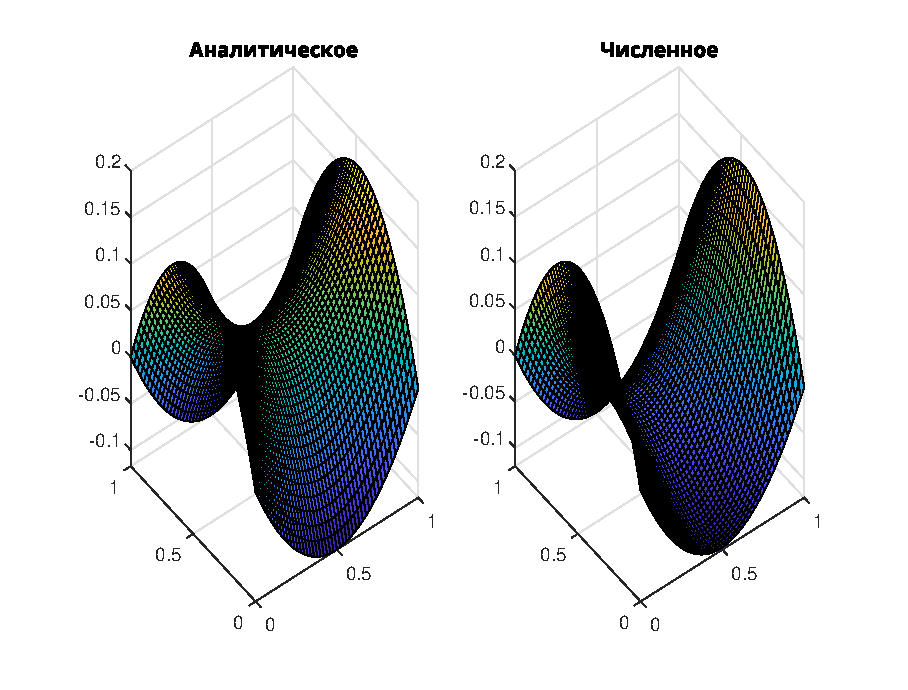
\includegraphics[width=1.1\textwidth, height=0.5\textheight]{12.eps}

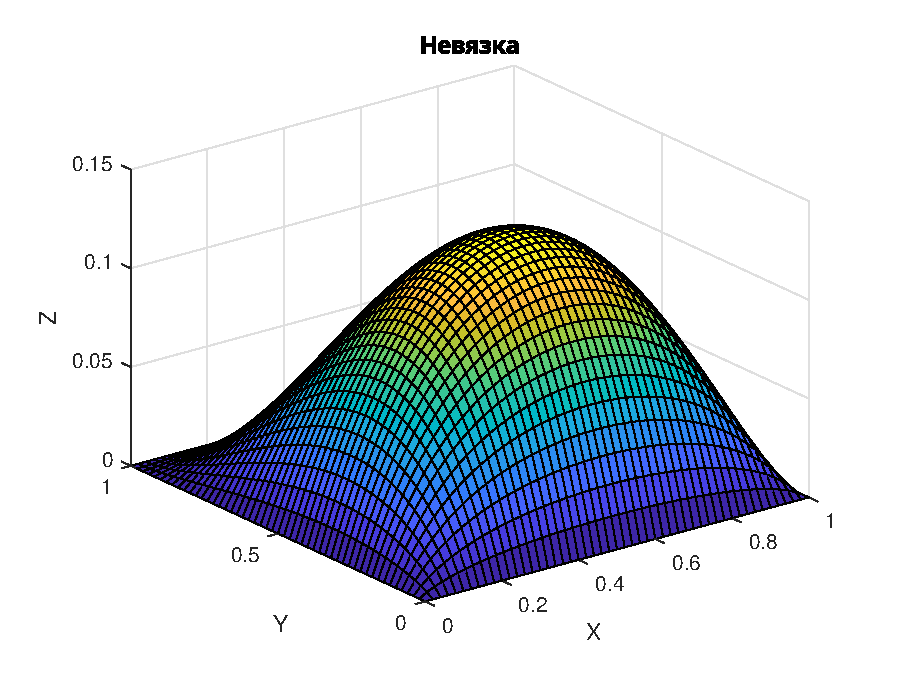
\includegraphics[width=0.7\textwidth]{11.eps}

\newpage
\subsection{$M = 50,\ N = 50,\ \mu= 100,\ u_1^0 = 1,\ u_2^0 = 1$}

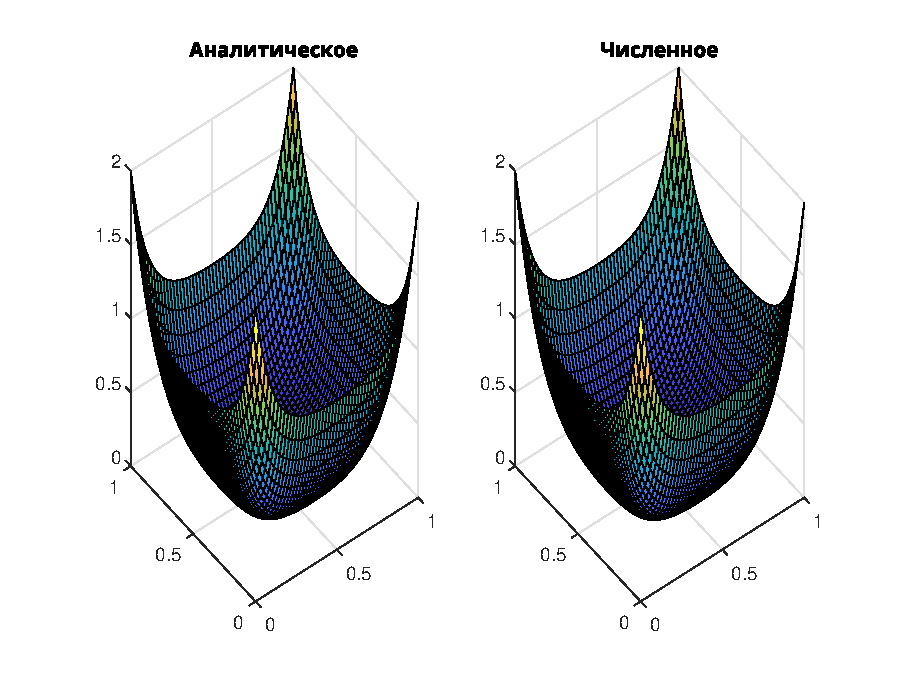
\includegraphics[width=1.1\textwidth, height=0.5\textheight]{22.eps}

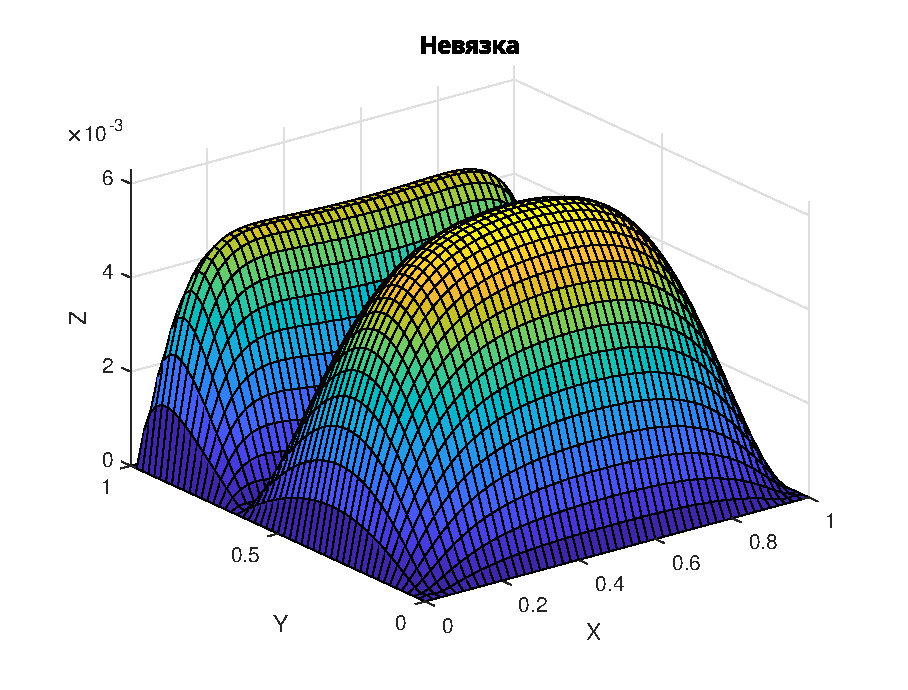
\includegraphics[width=0.7\textwidth]{21.eps}

\section{Решения для некоторых произвольных функций}
Рассмотрим численные решения для некоторых произвольных функций.

\subsection{$M = 40,\ N = 45,\ \mu= 120,\ f(x, y) = (x^2 + y^2)^2,\ \xi(x) = \sin(2\pi x),\ \eta(y) = \sin(-2\pi y)$}

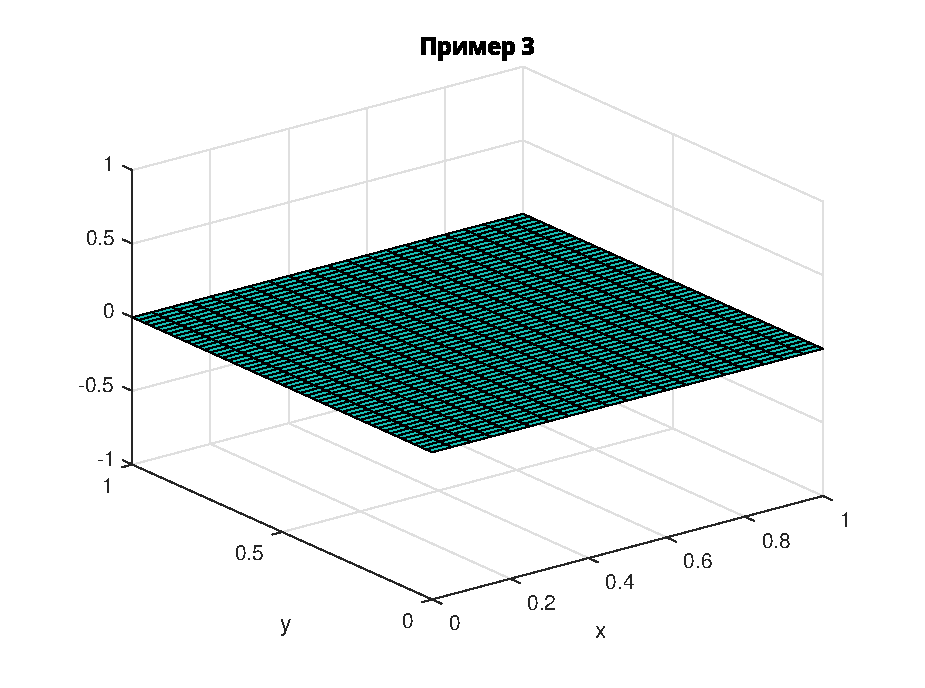
\includegraphics[width=0.7\textwidth]{3.eps}

\subsection{$M = 50,\ N = 50,\ \mu= 10,\ f(x, y) = 10\sin(xy),\ \xi(x) \equiv 0, \ \eta(y) \equiv 0$}

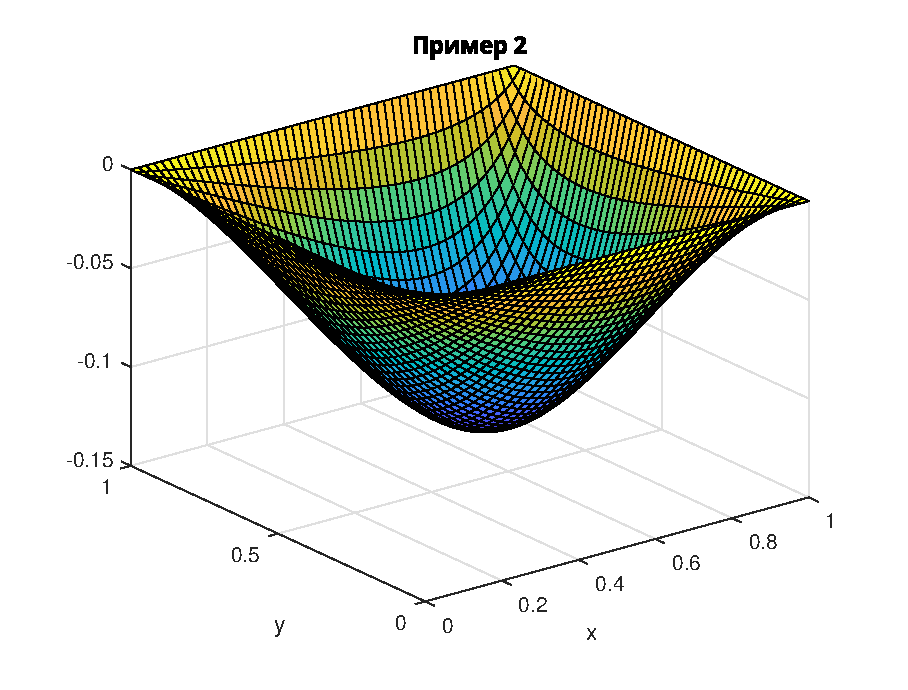
\includegraphics[width=0.7\textwidth]{4.eps}

\subsection{$M = 20,\ N = 50,\ \mu= 10,\ f(x, y) \equiv 0,\ \xi(x) \equiv 0, \ \eta(y) \equiv 0$}

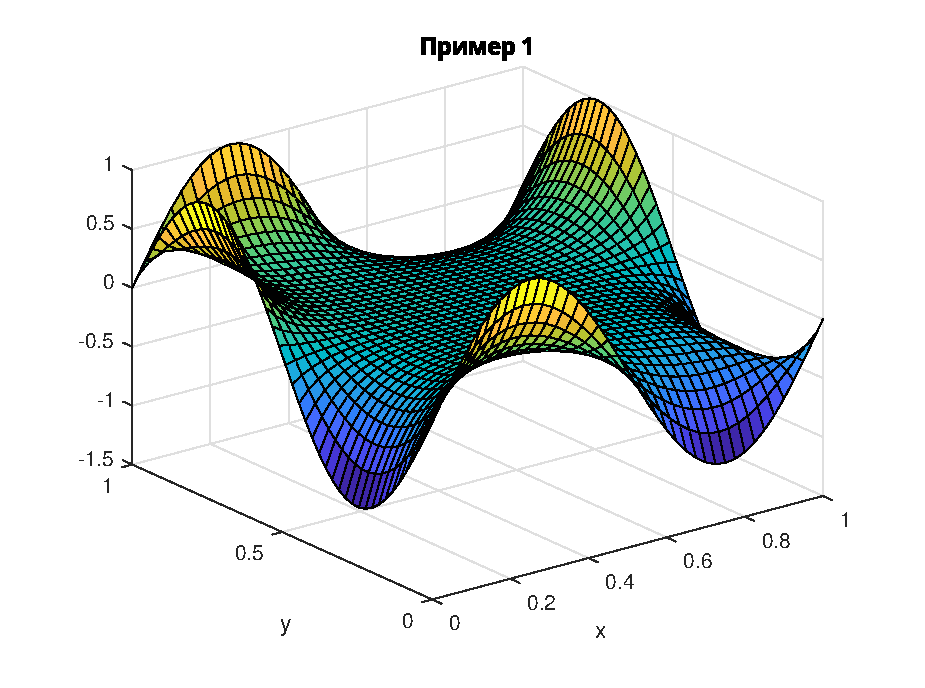
\includegraphics[width=0.7\textwidth]{5.eps}

\begin{thebibliography}{99}
\bibitem{1} Точилин П.А. Лекции по Преобразованиям Лапласа Фурье 2024
\end{thebibliography}

\end{document}


